\documentclass[twoside]{book}

% Packages required by doxygen
\usepackage{fixltx2e}
\usepackage{calc}
\usepackage{doxygen}
\usepackage[export]{adjustbox} % also loads graphicx
\usepackage{graphicx}
\usepackage[utf8]{inputenc}
\usepackage{makeidx}
\usepackage{multicol}
\usepackage{multirow}
\PassOptionsToPackage{warn}{textcomp}
\usepackage{textcomp}
\usepackage[nointegrals]{wasysym}
\usepackage[table]{xcolor}

% NLS support packages
\usepackage[T2A]{fontenc}
\usepackage[russian]{babel}

% Font selection
\usepackage[T1]{fontenc}
\usepackage[scaled=.90]{helvet}
\usepackage{courier}
\usepackage{amssymb}
\usepackage{sectsty}
\renewcommand{\familydefault}{\sfdefault}
\allsectionsfont{%
  \fontseries{bc}\selectfont%
  \color{darkgray}%
}
\renewcommand{\DoxyLabelFont}{%
  \fontseries{bc}\selectfont%
  \color{darkgray}%
}
\newcommand{\+}{\discretionary{\mbox{\scriptsize$\hookleftarrow$}}{}{}}

% Page & text layout
\usepackage{geometry}
\geometry{%
  a4paper,%
  top=2.5cm,%
  bottom=2.5cm,%
  left=2.5cm,%
  right=2.5cm%
}
\tolerance=750
\hfuzz=15pt
\hbadness=750
\setlength{\emergencystretch}{15pt}
\setlength{\parindent}{0cm}
\setlength{\parskip}{3ex plus 2ex minus 2ex}
\makeatletter
\renewcommand{\paragraph}{%
  \@startsection{paragraph}{4}{0ex}{-1.0ex}{1.0ex}{%
    \normalfont\normalsize\bfseries\SS@parafont%
  }%
}
\renewcommand{\subparagraph}{%
  \@startsection{subparagraph}{5}{0ex}{-1.0ex}{1.0ex}{%
    \normalfont\normalsize\bfseries\SS@subparafont%
  }%
}
\makeatother

% Headers & footers
\usepackage{fancyhdr}
\pagestyle{fancyplain}
\fancyhead[LE]{\fancyplain{}{\bfseries\thepage}}
\fancyhead[CE]{\fancyplain{}{}}
\fancyhead[RE]{\fancyplain{}{\bfseries\leftmark}}
\fancyhead[LO]{\fancyplain{}{\bfseries\rightmark}}
\fancyhead[CO]{\fancyplain{}{}}
\fancyhead[RO]{\fancyplain{}{\bfseries\thepage}}
\fancyfoot[LE]{\fancyplain{}{}}
\fancyfoot[CE]{\fancyplain{}{}}
\fancyfoot[RE]{\fancyplain{}{\bfseries\scriptsize Создано системой Doxygen }}
\fancyfoot[LO]{\fancyplain{}{\bfseries\scriptsize Создано системой Doxygen }}
\fancyfoot[CO]{\fancyplain{}{}}
\fancyfoot[RO]{\fancyplain{}{}}
\renewcommand{\footrulewidth}{0.4pt}
\renewcommand{\chaptermark}[1]{%
  \markboth{#1}{}%
}
\renewcommand{\sectionmark}[1]{%
  \markright{\thesection\ #1}%
}

% Indices & bibliography
\usepackage{natbib}
\usepackage[titles]{tocloft}
\setcounter{tocdepth}{3}
\setcounter{secnumdepth}{5}
\makeindex

% Hyperlinks (required, but should be loaded last)
\usepackage{ifpdf}
\ifpdf
  \usepackage[pdftex,pagebackref=true]{hyperref}
\else
  \usepackage[ps2pdf,pagebackref=true]{hyperref}
\fi
\hypersetup{%
  colorlinks=true,%
  linkcolor=blue,%
  citecolor=blue,%
  unicode%
}

% Custom commands
\newcommand{\clearemptydoublepage}{%
  \newpage{\pagestyle{empty}\cleardoublepage}%
}

\usepackage{caption}
\captionsetup{labelsep=space,justification=centering,font={bf},singlelinecheck=off,skip=4pt,position=top}

%===== C O N T E N T S =====

\begin{document}

% Titlepage & ToC
\hypersetup{pageanchor=false,
             bookmarksnumbered=true,
             pdfencoding=unicode
            }
\pagenumbering{alph}
\begin{titlepage}
\vspace*{7cm}
\begin{center}%
{\Large My Project }\\
\vspace*{1cm}
{\large Создано системой Doxygen 1.8.13}\\
\end{center}
\end{titlepage}
\clearemptydoublepage
\pagenumbering{roman}
\tableofcontents
\clearemptydoublepage
\pagenumbering{arabic}
\hypersetup{pageanchor=true}

%--- Begin generated contents ---
\chapter{Иерархический список классов}
\section{Иерархия классов}
Иерархия классов.\begin{DoxyCompactList}
\item \contentsline{section}{lex\+:\+:Divider}{\pageref{classlex_1_1_divider}}{}
\begin{DoxyCompactList}
\item \contentsline{section}{simple\+Divider}{\pageref{classsimple_divider}}{}
\end{DoxyCompactList}
\item \contentsline{section}{lex\+:\+:Lexer}{\pageref{classlex_1_1_lexer}}{}
\item \contentsline{section}{lex\+:\+:Token}{\pageref{classlex_1_1_token}}{}
\item \contentsline{section}{lex\+:\+:Tokenizer}{\pageref{classlex_1_1_tokenizer}}{}
\end{DoxyCompactList}

\chapter{Алфавитный указатель классов}
\section{Классы}
Классы с их кратким описанием.\begin{DoxyCompactList}
\item\contentsline{section}{\mbox{\hyperlink{classlex_1_1_divider}{lex\+::\+Divider}} \\*Виртуальный класс для создания разделителей }{\pageref{classlex_1_1_divider}}{}
\item\contentsline{section}{\mbox{\hyperlink{class_error}{Error}} }{\pageref{class_error}}{}
\item\contentsline{section}{\mbox{\hyperlink{classlex_1_1_lexer}{lex\+::\+Lexer}} \\*Класс лексического анализатора }{\pageref{classlex_1_1_lexer}}{}
\item\contentsline{section}{\mbox{\hyperlink{classsyntax_1_1_rule}{syntax\+::\+Rule}} }{\pageref{classsyntax_1_1_rule}}{}
\item\contentsline{section}{\mbox{\hyperlink{classsimple_divider}{simple\+Divider}} }{\pageref{classsimple_divider}}{}
\item\contentsline{section}{\mbox{\hyperlink{classsyntax_1_1_syntax}{syntax\+::\+Syntax}} }{\pageref{classsyntax_1_1_syntax}}{}
\item\contentsline{section}{\mbox{\hyperlink{classlex_1_1_token}{lex\+::\+Token}} \\*Класс для представления токенов }{\pageref{classlex_1_1_token}}{}
\item\contentsline{section}{\mbox{\hyperlink{classlex_1_1_tokenizer}{lex\+::\+Tokenizer}} \\*Класс Токенизатора }{\pageref{classlex_1_1_tokenizer}}{}
\item\contentsline{section}{\mbox{\hyperlink{classsyntax_1_1_tree}{syntax\+::\+Tree}} \\*Класс для представления бинарного дерева }{\pageref{classsyntax_1_1_tree}}{}
\item\contentsline{section}{\mbox{\hyperlink{class_word_tokenizer}{Word\+Tokenizer}} }{\pageref{class_word_tokenizer}}{}
\end{DoxyCompactList}

\chapter{Классы}
\hypertarget{classlex_1_1_divider}{}\section{Класс lex\+:\+:Divider}
\label{classlex_1_1_divider}\index{lex\+::\+Divider@{lex\+::\+Divider}}


Виртуальный класс для создания разделителей  




{\ttfamily \#include $<$lexer.\+h$>$}

Граф наследования\+:lex\+:\+:Divider\+:\begin{figure}[H]
\begin{center}
\leavevmode
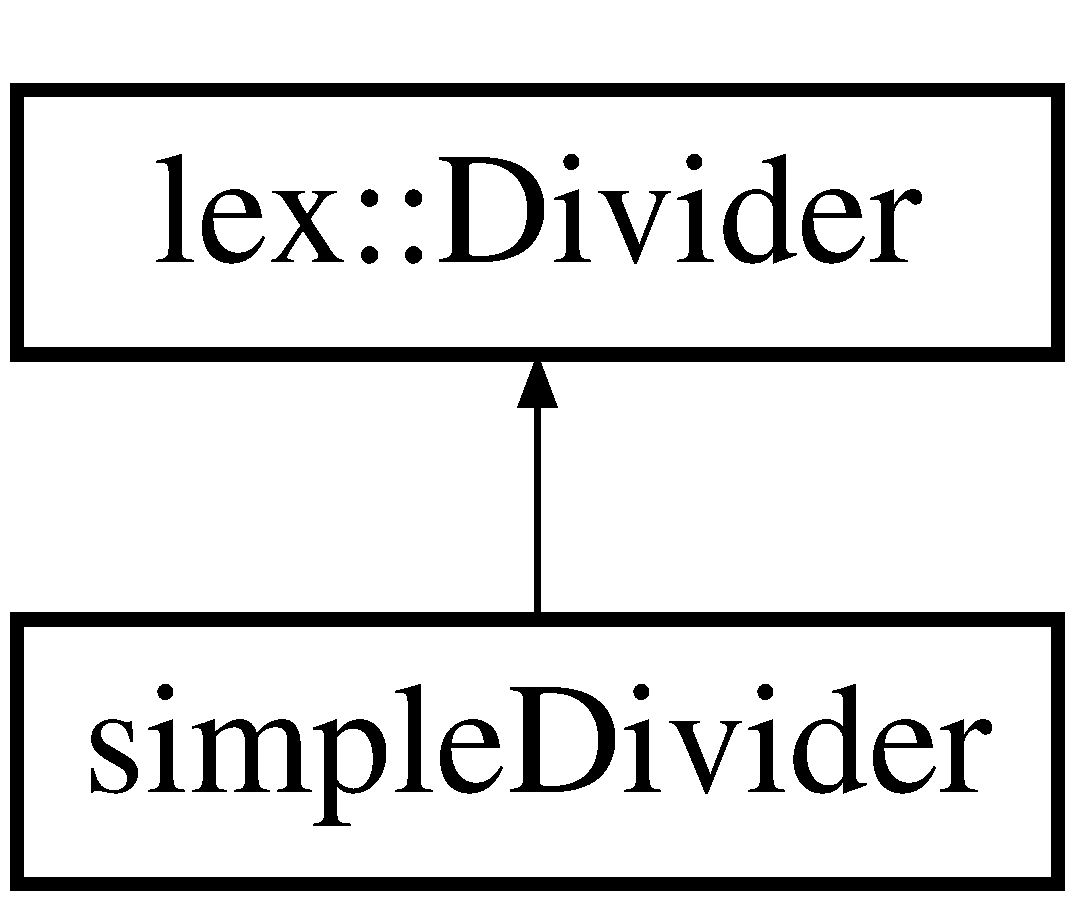
\includegraphics[height=2.000000cm]{classlex_1_1_divider}
\end{center}
\end{figure}
\subsection*{Открытые члены}
\begin{DoxyCompactItemize}
\item 
\mbox{\Hypertarget{classlex_1_1_divider_ac8cfe376aa8c0b04219b0512bfb6cb25}\label{classlex_1_1_divider_ac8cfe376aa8c0b04219b0512bfb6cb25}} 
virtual bool \mbox{\hyperlink{classlex_1_1_divider_ac8cfe376aa8c0b04219b0512bfb6cb25}{is\+Divide}} (char letter)=0
\begin{DoxyCompactList}\small\item\em Метод для разделения строк на лексемы \end{DoxyCompactList}\end{DoxyCompactItemize}


\subsection{Подробное описание}
Виртуальный класс для создания разделителей 

\begin{DoxyAuthor}{Автор}
grumgog 
\end{DoxyAuthor}
\begin{DoxyDate}{Дата}
27.\+06.\+2018 
\end{DoxyDate}
\begin{DoxyVersion}{Версия}
0.\+2
\end{DoxyVersion}
Разделитель -\/ специальный класс содержащий метод is\+Divide для разделения строки на лексемы. 

Объявления и описания членов класса находятся в файле\+:\begin{DoxyCompactItemize}
\item 
C\+:/\+Users/grumgog/\+Desktop/\+Work\+On/do\+Lang/src/lexer.\+h\end{DoxyCompactItemize}

\hypertarget{classlex_1_1_lexer}{}\section{Класс lex\+:\+:Lexer}
\label{classlex_1_1_lexer}\index{lex\+::\+Lexer@{lex\+::\+Lexer}}


Класс лексического анализатора  




{\ttfamily \#include $<$lexer.\+h$>$}

\subsection*{Открытые члены}
\begin{DoxyCompactItemize}
\item 
\mbox{\Hypertarget{classlex_1_1_lexer_a4c3c63439f64bf232e8995aaa555a7e4}\label{classlex_1_1_lexer_a4c3c63439f64bf232e8995aaa555a7e4}} 
{\bfseries Lexer} (\hyperlink{classlex_1_1_divider}{Divider} $\ast$div\+Obj, std\+::vector$<$ \hyperlink{classlex_1_1_tokenizer}{Tokenizer} $\ast$$>$ t=std\+::vector$<$ \hyperlink{classlex_1_1_tokenizer}{Tokenizer} $\ast$$>$())
\item 
\mbox{\Hypertarget{classlex_1_1_lexer_a64c1af615d7d401c0e6fcbf0c0c8e02b}\label{classlex_1_1_lexer_a64c1af615d7d401c0e6fcbf0c0c8e02b}} 
{\bfseries Lexer} (\hyperlink{classlex_1_1_divider}{Divider} $\ast$div\+Obj, \hyperlink{classlex_1_1_tokenizer}{Tokenizer} $\ast$one)
\item 
\mbox{\Hypertarget{classlex_1_1_lexer_a950c6154df77c2be981ae428d901eb48}\label{classlex_1_1_lexer_a950c6154df77c2be981ae428d901eb48}} 
void {\bfseries add\+Tokenizer} (\hyperlink{classlex_1_1_tokenizer}{Tokenizer} $\ast$t)
\item 
\mbox{\Hypertarget{classlex_1_1_lexer_aeb57d492b39419657a5f167317e7bc34}\label{classlex_1_1_lexer_aeb57d492b39419657a5f167317e7bc34}} 
void {\bfseries set\+Divider} (\hyperlink{classlex_1_1_divider}{Divider} $\ast$)
\item 
\mbox{\Hypertarget{classlex_1_1_lexer_a95cfd8a79f29edc132fb9cd66f3a0fe9}\label{classlex_1_1_lexer_a95cfd8a79f29edc132fb9cd66f3a0fe9}} 
std\+::vector$<$ std\+::string $>$ {\bfseries divide\+Lex} (std\+::string str, \hyperlink{classlex_1_1_divider}{Divider} $\ast$div\+Obj)
\item 
\mbox{\Hypertarget{classlex_1_1_lexer_a4ba2959182553e6ef14ec9f4ec717289}\label{classlex_1_1_lexer_a4ba2959182553e6ef14ec9f4ec717289}} 
std\+::vector$<$ \hyperlink{classlex_1_1_token}{Token} $>$ {\bfseries tokenize} (std\+::vector$<$ std\+::string $>$ lexs)
\end{DoxyCompactItemize}


\subsection{Подробное описание}
Класс лексического анализатора 

\begin{DoxyAuthor}{Автор}
grumgog 
\end{DoxyAuthor}
\begin{DoxyDate}{Дата}
27.\+06.\+2018 
\end{DoxyDate}
\begin{DoxyVersion}{Версия}
0.\+2
\end{DoxyVersion}
Лексический анализатор -\/ модуль занимающийся разбором строки на лексемы -\/ самостоятельные \char`\"{}слова\char`\"{} языка. Для определения токенов, нужно добавить токенизаторы -\/ унаследованные от \hyperlink{classlex_1_1_tokenizer}{Tokenizer}. Для правильного определения типа токена, рекомендуеться добавлять токенизаторы от более конкретного к более общему случаю. Например целые\+\_\+числа $<$-\/ вещественные\+\_\+числа 

Объявления и описания членов классов находятся в файлах\+:\begin{DoxyCompactItemize}
\item 
C\+:/\+Users/днс/\+Desktop/\+Work\+On/do\+Lang/src/lexer.\+h\item 
C\+:/\+Users/днс/\+Desktop/\+Work\+On/do\+Lang/src/lexer.\+cpp\end{DoxyCompactItemize}

\hypertarget{classsimple_divider}{}\section{Класс simple\+Divider}
\label{classsimple_divider}\index{simple\+Divider@{simple\+Divider}}
Граф наследования\+:simple\+Divider\+:\begin{figure}[H]
\begin{center}
\leavevmode
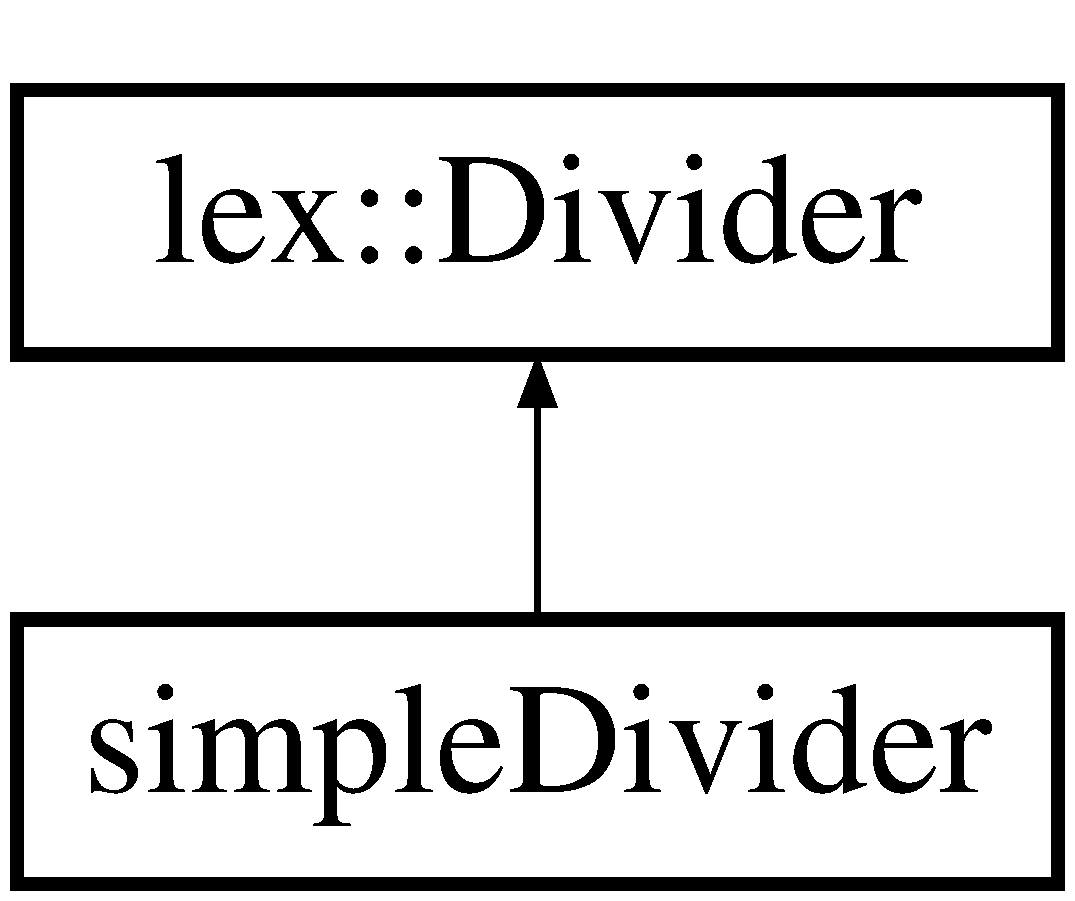
\includegraphics[height=2.000000cm]{classsimple_divider}
\end{center}
\end{figure}
\subsection*{Открытые члены}
\begin{DoxyCompactItemize}
\item 
\mbox{\Hypertarget{classsimple_divider_aa571e9a8bb1df785ac0f05ad16434241}\label{classsimple_divider_aa571e9a8bb1df785ac0f05ad16434241}} 
virtual bool \mbox{\hyperlink{classsimple_divider_aa571e9a8bb1df785ac0f05ad16434241}{is\+Divide}} (char letter)
\begin{DoxyCompactList}\small\item\em Метод для разделения строк на лексемы \end{DoxyCompactList}\end{DoxyCompactItemize}


Объявления и описания членов класса находятся в файле\+:\begin{DoxyCompactItemize}
\item 
C\+:/\+Users/grumgog/\+Desktop/\+Work\+On/do\+Lang/src/main.\+cpp\end{DoxyCompactItemize}

\hypertarget{classlex_1_1_token}{}\section{Класс lex\+:\+:Token}
\label{classlex_1_1_token}\index{lex\+::\+Token@{lex\+::\+Token}}


Класс для представления токенов  




{\ttfamily \#include $<$lexer.\+h$>$}

\subsection*{Открытые члены}
\begin{DoxyCompactItemize}
\item 
\mbox{\Hypertarget{classlex_1_1_token_a6c0d111952542890396445d9f693197f}\label{classlex_1_1_token_a6c0d111952542890396445d9f693197f}} 
{\bfseries Token} (Token\+Type t=Token\+Type\+::\+N\+O\+NE, std\+::string value=\char`\"{}\char`\"{})
\item 
\mbox{\Hypertarget{classlex_1_1_token_a2aecfe08aecdc1899502936dd8995a94}\label{classlex_1_1_token_a2aecfe08aecdc1899502936dd8995a94}} 
{\bfseries Token} (\hyperlink{classlex_1_1_token}{Token} \&t)
\item 
\mbox{\Hypertarget{classlex_1_1_token_ae4852777dbda0c82229172774e15a583}\label{classlex_1_1_token_ae4852777dbda0c82229172774e15a583}} 
\hyperlink{classlex_1_1_token}{Token} {\bfseries operator=} (\hyperlink{classlex_1_1_token}{Token} \&t)
\item 
\mbox{\Hypertarget{classlex_1_1_token_a0259f9e1504683176217e357101b5a68}\label{classlex_1_1_token_a0259f9e1504683176217e357101b5a68}} 
void {\bfseries set\+Type} (Token\+Type t)
\item 
\mbox{\Hypertarget{classlex_1_1_token_ab2e13a9b952b3afa6fe648d6b81e64a5}\label{classlex_1_1_token_ab2e13a9b952b3afa6fe648d6b81e64a5}} 
void {\bfseries set\+Value} (std\+::string v)
\item 
\mbox{\Hypertarget{classlex_1_1_token_a77574e198178aeb459865f304ce8c22e}\label{classlex_1_1_token_a77574e198178aeb459865f304ce8c22e}} 
Token\+Type {\bfseries get\+Type} ()
\item 
\mbox{\Hypertarget{classlex_1_1_token_a614cc525749151e1fcbcfdf9005b8c94}\label{classlex_1_1_token_a614cc525749151e1fcbcfdf9005b8c94}} 
std\+::string {\bfseries get\+Value} ()
\end{DoxyCompactItemize}


\subsection{Подробное описание}
Класс для представления токенов 

\begin{DoxyAuthor}{Автор}
grumgog 
\end{DoxyAuthor}
\begin{DoxyDate}{Дата}
27.\+06.\+2018 
\end{DoxyDate}
\begin{DoxyVersion}{Версия}
0.\+2 Токен -\/ пара значений $<$тип, значение$>$ 
\end{DoxyVersion}


Объявления и описания членов классов находятся в файлах\+:\begin{DoxyCompactItemize}
\item 
C\+:/\+Users/днс/\+Desktop/\+Work\+On/do\+Lang/src/lexer.\+h\item 
C\+:/\+Users/днс/\+Desktop/\+Work\+On/do\+Lang/src/lexer.\+cpp\end{DoxyCompactItemize}

\hypertarget{classlex_1_1_tokenizer}{}\section{Класс lex\+:\+:Tokenizer}
\label{classlex_1_1_tokenizer}\index{lex\+::\+Tokenizer@{lex\+::\+Tokenizer}}


Виртуальный класс для токенизаторов  




{\ttfamily \#include $<$lexer.\+h$>$}

\subsection*{Открытые члены}
\begin{DoxyCompactItemize}
\item 
\mbox{\Hypertarget{classlex_1_1_tokenizer_a6fd22f79c30b936923c2e408eaaf835c}\label{classlex_1_1_tokenizer_a6fd22f79c30b936923c2e408eaaf835c}} 
virtual \hyperlink{classlex_1_1_token}{Token} {\bfseries analysis} (std\+::string lex)=0
\end{DoxyCompactItemize}


\subsection{Подробное описание}
Виртуальный класс для токенизаторов 

\begin{DoxyAuthor}{Автор}
grumgog 
\end{DoxyAuthor}
\begin{DoxyDate}{Дата}
27.\+06.\+2018 
\end{DoxyDate}
\begin{DoxyVersion}{Версия}
0.\+2
\end{DoxyVersion}
Токенизатор -\/ класс для определения типа лексемы. один тип -\/ один токенизатор 

Объявления и описания членов класса находятся в файле\+:\begin{DoxyCompactItemize}
\item 
C\+:/\+Users/днс/\+Desktop/\+Work\+On/do\+Lang/src/lexer.\+h\end{DoxyCompactItemize}

%--- End generated contents ---

% Index
\backmatter
\newpage
\phantomsection
\clearemptydoublepage
\addcontentsline{toc}{chapter}{Алфавитный указатель}
\printindex

\end{document}
